\section{Requerimientos Funcionales}

\section{Requerimientos No Funcionales}

\section{Reglas de Negocio}

\section{Diagramas de Casos de Uso}
	En esta sección se presentan los casos de uso diseñados con base en los RF, RNF y RN. Están ordenados por módulos del sistema.
	
	\subsection{Módulo de Gestión de Usuarios}
	El módulo de Gestión de Usuarios poseé los siguientes casos de uso.
	
		\subsubsection{CU2: Dar de alta empleado del CMPL}
			\begin{figure}[htbp!]
				\centering
					%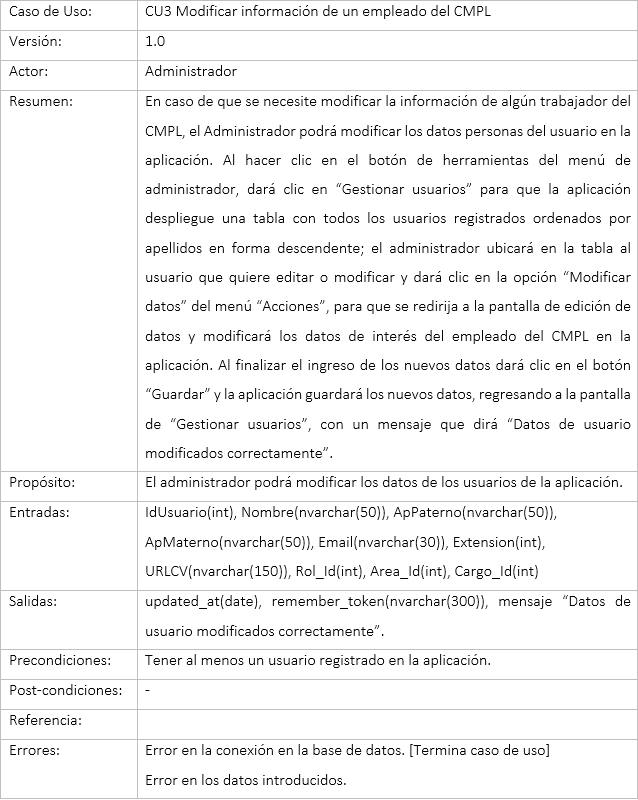
\includegraphics[width=0.8\textwidth]{images/CU/CU3}
					\caption{Caso de uso 2: Dar de alta empleado del CMPL.}
				\label{Tabla}
			\end{figure}
			
			\begin{itemize}
				\item Trayectoria principal:
					\begin{enumerate}
						\item El actor va a la sección de correspondencia 
					\end{enumerate}
				\item Trayectorias alternativas:
					\begin{itemize}
						\item Trayectoria alternativa A:
							\begin{enumerate}
								\item La aplicación muestra un mensaje de error.
							\end{enumerate}
					\end{itemize}
			\end{itemize}
			
		\subsubsection{CU3: Modificar información de un empleado del CMPL}
			\begin{figure}[htbp!]
				\centering
					%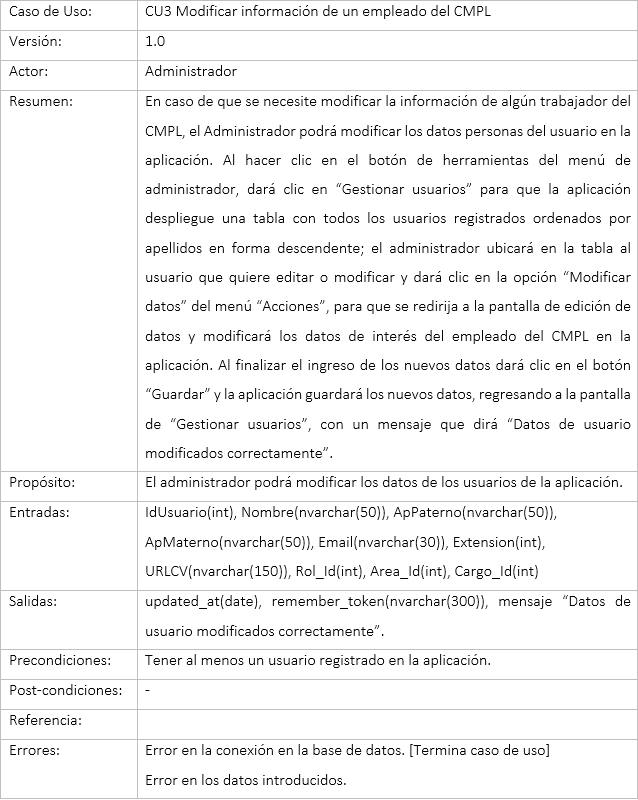
\includegraphics[width=0.8\textwidth]{images/CU/CU3}
					\caption{Caso de uso 3: Modificar información de un empleado del CMPL.}
				\label{Tabla}
			\end{figure}
			
			\begin{itemize}
				\item Trayectoria principal:
					\begin{enumerate}
						\item El actor va a la sección de correspondencia 
					\end{enumerate}
				\item Trayectorias alternativas:
					\begin{itemize}
						\item Trayectoria alternativa A:
							\begin{enumerate}
								\item La aplicación muestra un mensaje de error.
							\end{enumerate}
					\end{itemize}
			\end{itemize}
		
		\subsubsection{CU4: Desactivar cuenta de usuario}
			\begin{figure}[htbp!]
				\centering
					%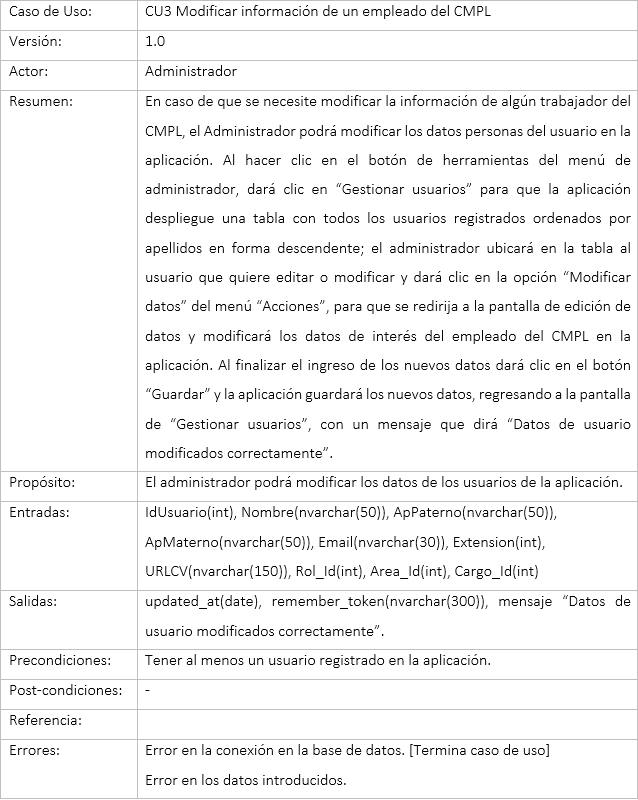
\includegraphics[width=0.8\textwidth]{images/CU/CU3}
					\caption{Caso de uso 4: Desactivar cuenta de usuario.}
				\label{Tabla}
			\end{figure}
			
			\begin{itemize}
				\item Trayectoria principal:
					\begin{enumerate}
						\item El actor va a la sección de correspondencia 
					\end{enumerate}
				\item Trayectorias alternativas:
					\begin{itemize}
						\item Trayectoria alternativa A:
							\begin{enumerate}
								\item La aplicación muestra un mensaje de error.
							\end{enumerate}
					\end{itemize}
			\end{itemize}
			
		\subsubsection{CU5: Activar cuenta de usuario}
			\begin{figure}[htbp!]
				\centering
					%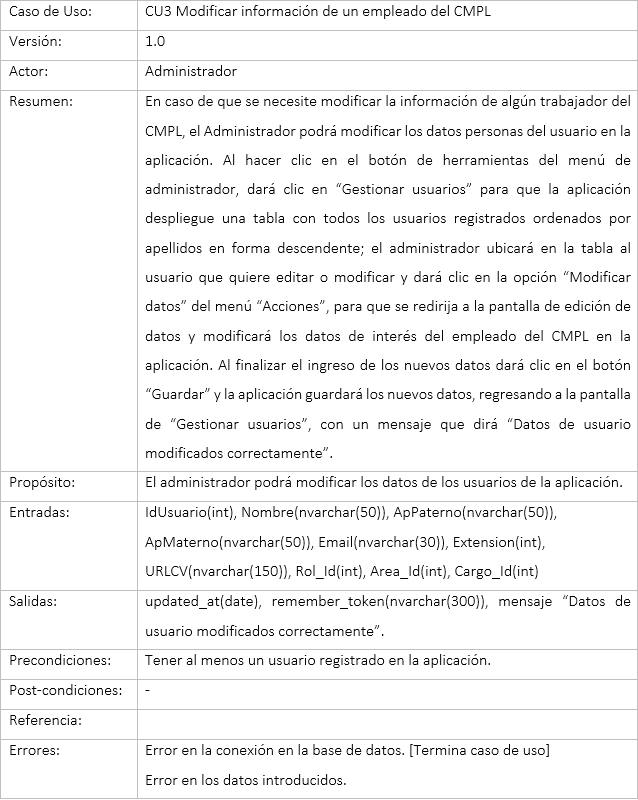
\includegraphics[width=0.8\textwidth]{images/CU/CU3}
					\caption{Caso de uso 5: Activar cuenta de usuario.}
				\label{Tabla}
			\end{figure}
			
			\begin{itemize}
				\item Trayectoria principal:
					\begin{enumerate}
						\item El actor va a la sección de correspondencia 
					\end{enumerate}
				\item Trayectorias alternativas:
					\begin{itemize}
						\item Trayectoria alternativa A:
							\begin{enumerate}
								\item La aplicación muestra un mensaje de error.
							\end{enumerate}
					\end{itemize}
			\end{itemize}
			
		\subsubsection{CU6: Ver directorio interno del CMPL}
			\begin{figure}[htbp!]
				\centering
					%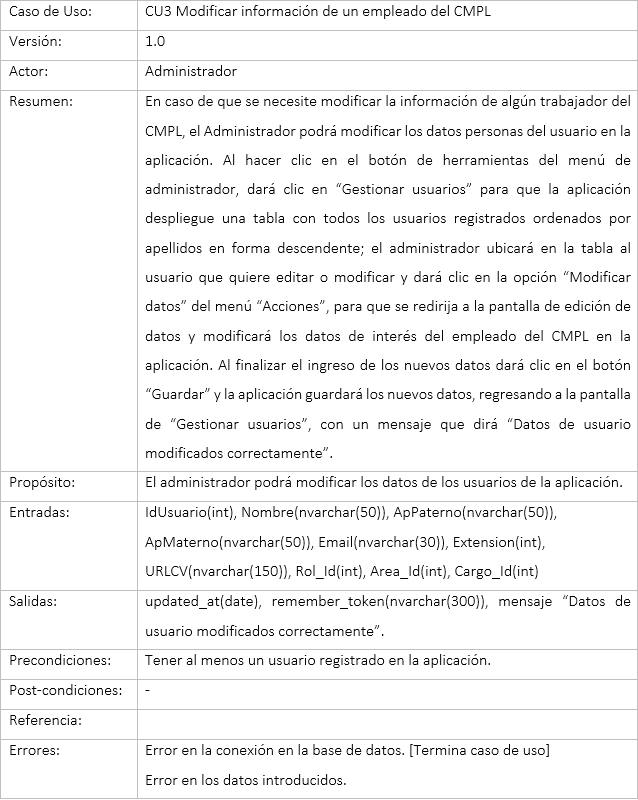
\includegraphics[width=0.8\textwidth]{images/CU/CU3}
					\caption{Caso de uso 6: Ver directorio interno del CMPL.}
				\label{Tabla}
			\end{figure}
			
			\begin{itemize}
				\item Trayectoria principal:
					\begin{enumerate}
						\item El actor va a la sección de correspondencia 
					\end{enumerate}
				\item Trayectorias alternativas:
					\begin{itemize}
						\item Trayectoria alternativa A:
							\begin{enumerate}
								\item La aplicación muestra un mensaje de error.
							\end{enumerate}
					\end{itemize}
			\end{itemize}
			
		\subsubsection{CU7: Ver directorio interno del CMPL por área o departamento}
			\begin{figure}[htbp!]
				\centering
					%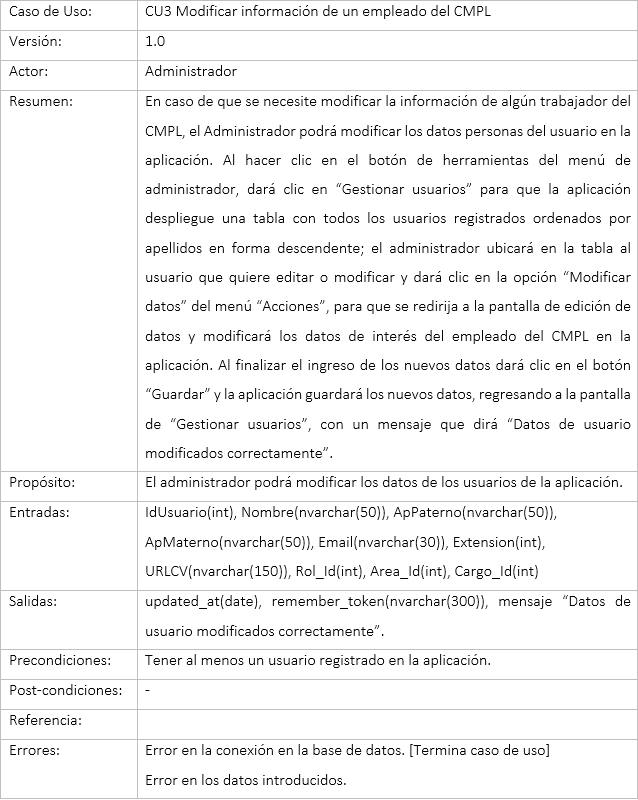
\includegraphics[width=0.8\textwidth]{images/CU/CU3}
					\caption{Caso de uso 7: Ver directorio interno del CMPL por área o departamento.}
				\label{Tabla}
			\end{figure}
			
			\begin{itemize}
				\item Trayectoria principal:
					\begin{enumerate}
						\item El actor va a la sección de correspondencia 
					\end{enumerate}
				\item Trayectorias alternativas:
					\begin{itemize}
						\item Trayectoria alternativa A:
							\begin{enumerate}
								\item La aplicación muestra un mensaje de error.
							\end{enumerate}
					\end{itemize}
			\end{itemize}
			
		\subsubsection{CU8: Buscar empleado del CMPL por nombre}
			\begin{figure}[htbp!]
				\centering
					%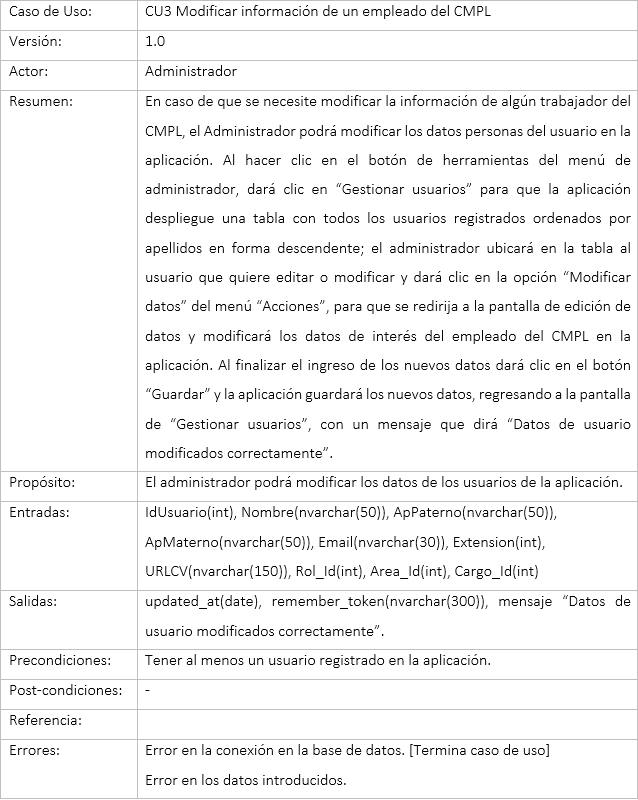
\includegraphics[width=0.8\textwidth]{images/CU/CU3}
					\caption{Caso de uso 8: Buscar empleado del CMPL por nombre.}
				\label{Tabla}
			\end{figure}
			
			\begin{itemize}
				\item Trayectoria principal:
					\begin{enumerate}
						\item El actor va a la sección de correspondencia 
					\end{enumerate}
				\item Trayectorias alternativas:
					\begin{itemize}
						\item Trayectoria alternativa A:
							\begin{enumerate}
								\item La aplicación muestra un mensaje de error.
							\end{enumerate}
					\end{itemize}
			\end{itemize}
			
		\subsubsection{CU9: Restablecer contraseña de usuario}
			\begin{figure}[htbp!]
				\centering
					%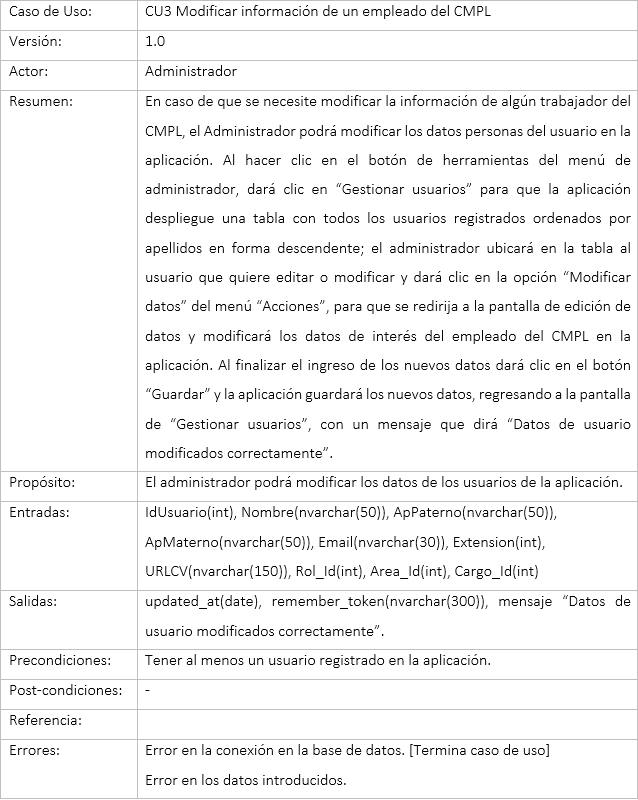
\includegraphics[width=0.8\textwidth]{images/CU/CU3}
					\caption{Caso de uso 9: Restablecer contraseña de usuario.}
				\label{Tabla}
			\end{figure}
			
			\begin{itemize}
				\item Trayectoria principal:
					\begin{enumerate}
						\item El actor va a la sección de correspondencia 
					\end{enumerate}
				\item Trayectorias alternativas:
					\begin{itemize}
						\item Trayectoria alternativa A:
							\begin{enumerate}
								\item La aplicación muestra un mensaje de error.
							\end{enumerate}
					\end{itemize}
			\end{itemize}
			
		\subsubsection{CU10: Modificar datos personales de usuario (Administrador)}
			\begin{figure}[htbp!]
				\centering
					%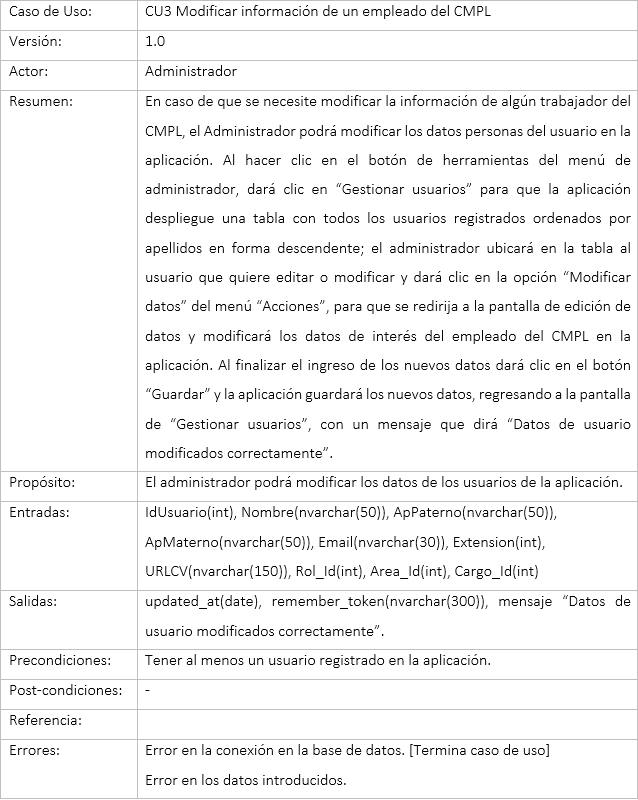
\includegraphics[width=0.8\textwidth]{images/CU/CU3}
					\caption{Caso de uso 10: Modificar datos personales de usuario (Administrador).}
				\label{Tabla}
			\end{figure}
			
			\begin{itemize}
				\item Trayectoria principal:
					\begin{enumerate}
						\item El actor va a la sección de correspondencia 
					\end{enumerate}
				\item Trayectorias alternativas:
					\begin{itemize}
						\item Trayectoria alternativa A:
							\begin{enumerate}
								\item La aplicación muestra un mensaje de error.
							\end{enumerate}
					\end{itemize}
			\end{itemize}
			
		\subsubsection{CU11: Modificar datos personales de usuario (Empleado del CMPL)}
			\begin{figure}[htbp!]
				\centering
					%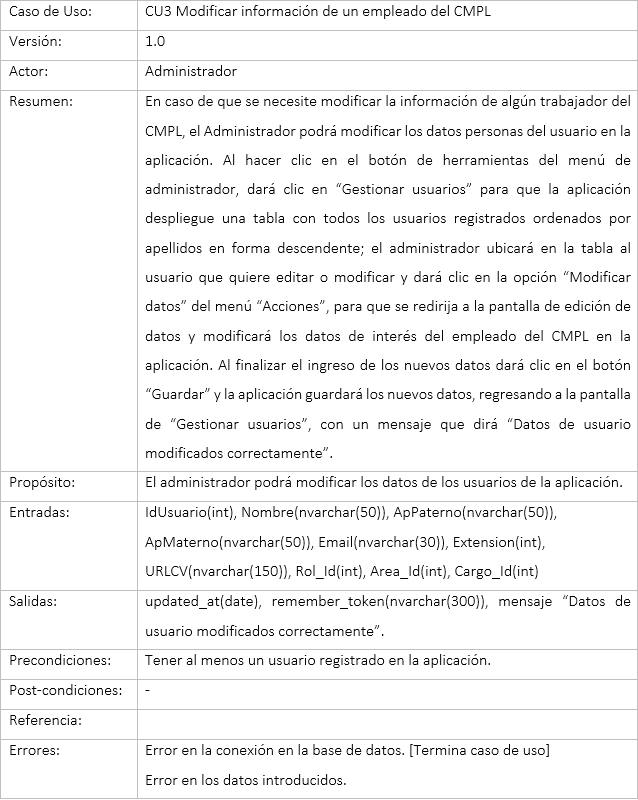
\includegraphics[width=0.8\textwidth]{images/CU/CU3}
					\caption{Caso de uso 11: Modificar datos personales de usuario (Empleado del CMPL).}
				\label{Tabla}
			\end{figure}
			
			\begin{itemize}
				\item Trayectoria principal:
					\begin{enumerate}
						\item El actor va a la sección de correspondencia 
					\end{enumerate}
				\item Trayectorias alternativas:
					\begin{itemize}
						\item Trayectoria alternativa A:
							\begin{enumerate}
								\item La aplicación muestra un mensaje de error.
							\end{enumerate}
					\end{itemize}
			\end{itemize}
			
		\subsubsection{CUn: }
			\begin{figure}[htbp!]
				\centering
					%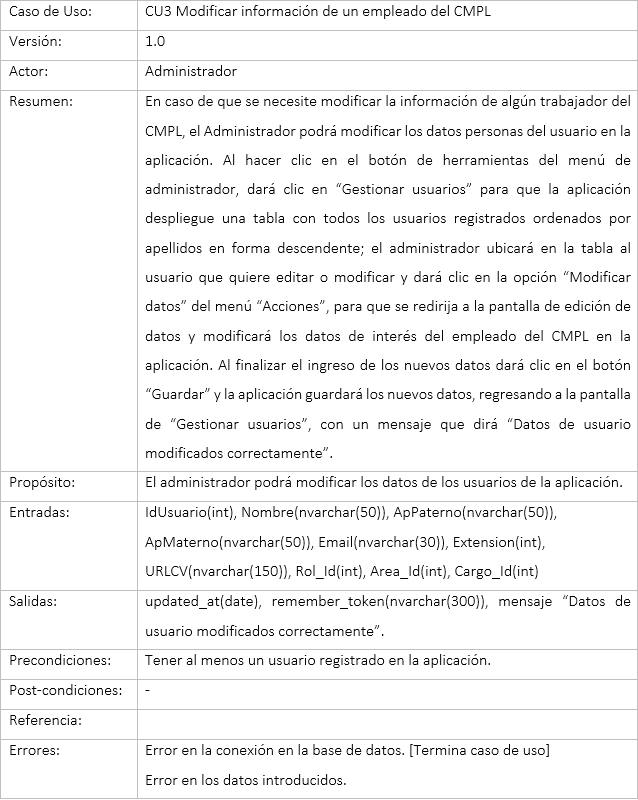
\includegraphics[width=0.8\textwidth]{images/CU/CU3}
					\caption{Caso de uso n: .}
				\label{Tabla}
			\end{figure}
			
			\begin{itemize}
				\item Trayectoria principal:
					\begin{enumerate}
						\item El actor va a la sección de correspondencia 
					\end{enumerate}
				\item Trayectorias alternativas:
					\begin{itemize}
						\item Trayectoria alternativa A:
							\begin{enumerate}
								\item La aplicación muestra un mensaje de error.
							\end{enumerate}
					\end{itemize}
			\end{itemize}

A continuación se muestran los casos de uso para los oficios salientes.
\begin{figure}[htbp!]
		\centering
			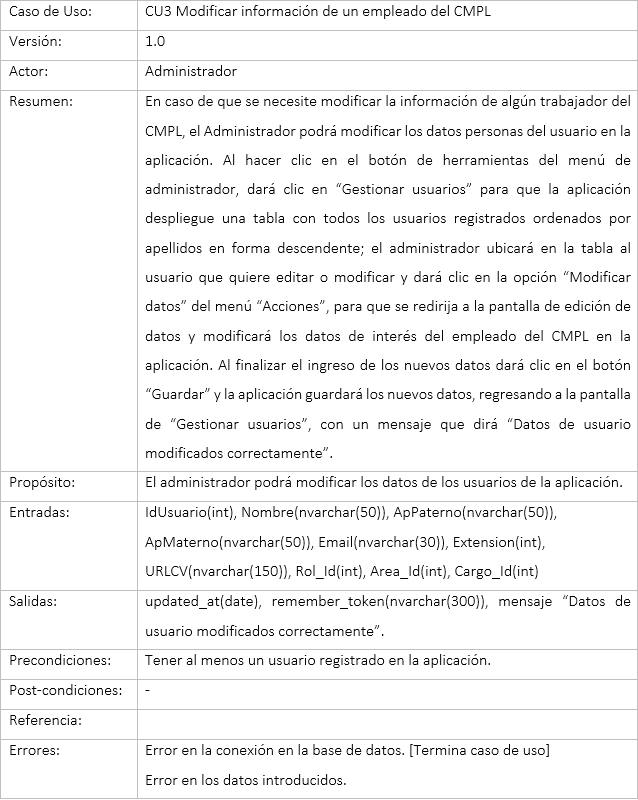
\includegraphics[width=0.8\textwidth]{images/CU/CU3}
		\caption{Caso de uso 3: Registrar oficio saliente.}
		\label{Tabla}
	\end{figure}

\begin{itemize}
	\item Trayectoria principal:
	\begin{enumerate}
		\item El actor va a la sección de correspondencia 
		\item La aplicación muestra la pantalla IU4 Correspondencia.
		\item El actor presiona el botón “Nuevo oficio”.
		\item La aplicación muestra la interfaz IU4.1 para el registro de oficios.
		\item El actor introduce los datos requeridos para el registro del oficio.
		\item El actor presiona el botón “Adjuntar documento”.
		\item CU27 Guardar Archivo.
		\item El usuario presiona el botón “Registrar”. 
		\item La aplicación hace la validación de los datos introducidos. [Trayectoria alternativa A] 
		\item La aplicación muestra el mensaje MSG2 de que el registro se realizó de forma exitosa.
		\item Fin del caso de uso.
	\end{enumerate}
	
	\item Trayectorias alternativas:
	\begin{itemize}
		\item Trayectoria alternativa A:
			\begin{enumerate}
				\item La aplicación muestra un mensaje de error.
				\item La aplicación resalta los campos en el formulario con errores.
				\item El usuario corrige los errores en el formulario.
				\item Continua en trayectoria del CU3 en paso 8.
			\end{enumerate}
	\end{itemize}
\end{itemize}

